\subsection{Orientering af SIFT punkter}
Formålet ved dette skridt er at estimere orienteringer af de detekterede punkter.
Orienteringen af et detekteret punkt anvendes af deskriptoren, for at opnå invarians overfor rotation. Orienteringen kan beskrives ved:
\begin{equation}
Orientering(p, \sigma) = \theta
\end{equation}
Hvor $p$ er interessepunktet, $\sigma$ er skalaen hvor interessepunktet er detekteret, og $\theta$ er orienteringen af punktet. 
\\
\\
Et $16\times16$ dataindsamlingsvindue placeres omkring et interessepunkt, på skalabilledet som interessepunktet er fundet på. For alle punkter i dataindsamlingsvinduet, er størrelsen på punkternes gradient, og deres orientering beregnet ved:
\begin{equation}
m(x,y) = \sqrt{(L(x + 1, y) - L(x - 1, y))^2 + (L(x, y + 1) - L(x, y - 1))^2} 
\label{magnitudepoint}
\end{equation}
\begin{equation}o(x,y) = tan^{-1}((L(x,y+1) - L(x,y-1))/(L(x+1, y) - L(x-1, y))) 
\label{orientationpoint}
\end{equation}
$m$ er størrelsen af en gradient, og $o$ er gradientens retning. For alle punkter indenfor dataindsamlingsvinduet, udregnes ligning
\eqref{magnitudepoint}, \eqref{orientationpoint}, og danner et gradientvindue $g$ og orienteringsvindue $v$, begge vinduer af størrelse $16\times16$. Gradientvinduet skal herefter foldes med et Gaussisk filter hvor $\sigma_{Gauss} = 1.5 \cdot \sigma_{point}$, med størrelse $16\times16$. Dette udføres for at vægte gradienter nær punktet højere end punkter i udkanten af vinduet.
\\
\\
Der oprettes derefter et orienteringshistogram $H$, med 36 indgange. Orienteringerne angivet i $v$ skal tilføjes histogrammet, vægtet af gradientstyrken angivet i $g$. En indgang i $H$, dækker en vinkel på $10^{\circ}$. F.eks. skal alle gradienter med vinkler mellem  $0^{\circ}-10^{\circ}$, tilføjes vægtet, til $H_1$, osv. Dette resulterer i et orienteringshistogram, hvor indgangen i histogrammet, med størst værdi, bliver bearbejdet. Lowe foreslår, at alle indgange i histogrammet, der ligger indenfor 80\% af det højeste punkt, bliver nye features - dette er undladt her, for at undgå at få for mange features. <Måske nævn empirisk op til 10 orienteringer ekstra per punkt!>
\\
Der skal nu foretages en interpolation, omkring den indgang i histogrammet, med størst værdi, for at få et mere præcist estimat af $\theta$.
\begin{figure}[H]
    \centering
    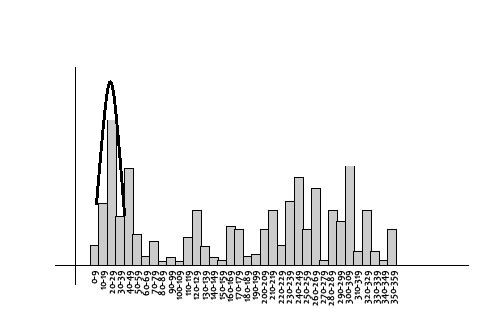
\includegraphics[width=0.60\textwidth]{fig/sift-orientation-histogram.jpg}
     \vspace{-1em}
    \begin{center}    
       \caption{\textcolor{gray}{\footnotesize \textit{Histogrammet $H$ afbilledet, sammen med en andengradsligning. Andengradsligningen er beregnet over den største indgang i $H$}}}
    \label{histogramheight}
     \end{center}
     \vspace{-2.5em}
  \end{figure} \noindent
Dette ses på figur \ref{histogramheight}, hvor et andengradspolynomium er blevet tilnærmet den største værdi af $H$. Estimering af andengradspolynomiet sker over den største værdi i $H$, og dens venstre og højre nabo.
\subsection*{Algoritme}
\textbf{Input} : Ét punkt og en skala, hvor punktet er lokaliseret $(x,y,\sigma)$  \\
\textbf{Output:} En orientering af punktet $\theta$.  \\
\begin{enumerate}
\item Placer dataindsamlingsvindue omkring  interessepunktet, på samme skalabillede som $\sigma$ foreskriver.
\item Anvend ligning \eqref{magnitudepoint}, \eqref{orientationpoint}, på hvert punkt i dataindsamlingsvinduet, for at udregne alle størrelser af orienteringer og gradienter. Gradientbilledet foldes derefter med et Gaussisk filter: $g = G(x,y,1.5 \cdot \sigma)$.
\item Adder værdierne i $g$ på indgange i histogrammet $H$, afhængigt af deres tilsvarede orientering i $v$.
\item  Udfør en interpolation omkring den største værdi i $H$ og to naboer. Denne værdi returneres.
\end{enumerate}
